\documentclass[a4paper]{report}
\usepackage[a4paper, left=1.3in, right=1.3in, top=1in, bottom=1in]{geometry}
\usepackage{tabularx}
\usepackage{amsmath}
\usepackage{graphicx}
\usepackage{subcaption}
\usepackage{cite}

\usepackage[utf8]{inputenc}
\usepackage[T1]{fontenc}
\usepackage{float}
\usepackage{multirow}
\usepackage{listings}
\usepackage{array}
\newcolumntype{P}[1]{>{\centering\arraybackslash}p{#1}}

\usepackage{indentfirst}
\usepackage{tensor}
\usepackage{amssymb}
\allowdisplaybreaks
\usepackage{bm}
\newcommand{\at}[2][]{#1|_{#2}}
\newcommand\numberthis{\addtocounter{equation}{1}\tag{\theequation}}
\newcommand\norm[1]{\left\lVert#1\right\rVert}
\usepackage{caption}
\captionsetup[lstlisting]{font={small}}
\captionsetup[figure]{font=small}
\captionsetup[table]{font=small}
\usepackage{breqn}
\usepackage{verbatim}


\usepackage[dvipsnames]{xcolor}
\usepackage{wrapfig}
\usepackage{hyperref}  % importare per ultimo https://www.overleaf.com/learn/latex/Hyperlinks
\definecolor{dkgrey}{rgb}{0.2, 0.2, 0.2}
\hypersetup{
    colorlinks=true,
    linkcolor=dkgrey,
    urlcolor=cyan,
		pdftitle={Report of C3AE Project},
}
\graphicspath{ {./images} }
% collegamento ipertestuale che scrive anche nome e numero del capitolo/sezione.
% Source: https://tex.stackexchange.com/questions/121865/nameref-how-to-display-section-name-and-its-number
\newcommand*{\fullref}[1]{\hyperref[{#1}]{\autoref*{#1}: \nameref*{#1}}}

\setlength{\parindent}{0pt}

\begin{document}

\title{Report of C3AE Project}

\makeatletter
\let\thetitle\@title
\let\theauthor\@author
\let\thedate\@date
\makeatother

\begin{titlepage}
	\centering
    \vspace*{0.5 cm}
    
\includegraphics{images/sapienza-MLred-pos}\\[1.0 cm]	% University Logo
    \vspace*{-0.3cm}
    \textsc{\large Facoltà di \\Ingegneria dell'Informazione, Informatica e Statistica}\\[0.5 cm]	% Department Name
    \textsc{\large Dipartimento \\di Ingegneria Informatica, Automatica e Gestionale}\\[0.5 cm]	% Department Name
    \textbf{\large Neural Networks course}\\[0.1 cm]
    \textbf{\large Final project}\\[2.0 cm]
    \textsc{\large A.Y. 2020/21}\\[2.0 cm]
    { \fontsize{20.74pt}{18.5pt}\selectfont\bfseries \thetitle \par } % title
    \vspace*{5.6cm}
	\begin{minipage}{0.4\textwidth}
		\begin{flushleft} \large
			\emph{Professors:}\\
			Aurelio Uncini\\
            Simone Scardapane
		\end{flushleft}
	\end{minipage}~
	\begin{minipage}{0.4\textwidth}
		\begin{flushright} \large
			\emph{Students:} \\
            Francesco Petri 1797147\\
            Giovanni Pecorelli 1799865
		\end{flushright}
	\end{minipage}\\[2 cm]
\end{titlepage}



\tableofcontents
\newpage

\setlength{\parskip}{1em}

%!TEX root = report.tex

\chapter{Introduction}
In the past decade soft biometrics has emerged out to be a new area of interest for the researchers due to its growing real-world 
applications. This includes a classic learning problem in computer vision: the estimation of demographic traits, such as the age. 
Researchers are trying to develop models which can accurately estimate the age or the age group of a person using different 
biometric traits. Currently, neural networks give the best classification results for age estimation using human faces.
Many CNNs (convolutional neural networks) such as AlexNet, VggNet, GoogLeNet and ResNet are able to accomplish this task with promising 
performance.\

However, to obtain more precise accuracy these networks have grown deeper and larger. This trend has resulted in increasingly higher 
computational costs in either training or deploying. In particular, deploying the previously mentioned models on mobile phones, cars and 
robots is next to impossible due to the model size and computational cost.\\
Recently other models have been proposed with the aim to reduce the number of parameters, thus yielding lightweight models without 
weakening their efficience.

In this work we want to investigate the limits of compact models for small-scale images and focus on one the most compact models for age 
classification, implementing it in practice to evaluate its performance.\\
The following report presents the development of the final project for the Neural Networks course at Università degli studi di Roma 
"La Sapienza", A.Y. 2020/21.

\section{Related works}

Our work is based on the study made by Chao Zhang, Shuaicheng Liu, Xun Xu and Ce Zhu in the paper \textit{"C3AE: Exploring the Limits 
of Compact Model for Age Estimation"} \cite{c3ae} in which they propose a \textbf{C}ompact basic model, \textbf{C}ascaded training 
and multi-scale \textbf{C}ontext, aiming to tackle small-scale image \textbf{A}ge \textbf{E}stimation. The model is called \textbf{C3AE}.

The proposed model is able to achieve a state-of-the-art performance compared with alternative compact models and even outperforms many 
bulky models. With an extremely compact size of 0.25 MB for the full model, which is possibly the smallest that has been
obtained so far on the facial recognition, C3AE is suitable to be deployed even on low-end mobiles and embedded platforms.

\section{Report organization}
This report is structured as follows:
\begin{itemize}
    \item In Chapter 2 we describe the datasets used for the training and the evaluation of the model, as well as the preprocessing 
      and the augmentation techniques used on them.
    \item In Chapter 3 we present the theory behind C3AE, explaining its model composition and our implementation.
    \item ... 
  \end{itemize}

%!TEX root = report.tex

\chapter{Datasets}
Donec id lacus venenatis, molestie lorem nec, commodo erat. Aliquam scelerisque sollicitudin diam, nec finibus lacus faucibus vitae. Pellentesque sapien est, volutpat non velit vel, eleifend tempus turpis. Aenean vehicula pretium lectus, ac consequat mi pretium at. Aliquam quis elit quam. Vestibulum ante ipsum primis in faucibus orci luctus et ultrices posuere cubilia curae; Nulla ornare, diam sed convallis sodales, dui lectus lobortis mauris, eu faucibus urna lacus eu metus. Quisque vitae varius risus. Ut a lacus sit amet massa iaculis elementum id quis ante. Vestibulum imperdiet ante erat, eget gravida purus condimentum ut. In a leo sed ligula placerat vulputate eget eget turpis. Mauris justo risus, sodales commodo nibh at, pulvinar facilisis leo. Donec vel condimentum nibh. Nullam ac mi nec felis pellentesque vulputate. Nulla facilisi.
\section{Preprocessing}
pppppppp
\section{Augmentation}
lllllll

%!TEX root = report.tex

\chapter{Theory Stuff}
Morbi maximus dui vitae lorem pretium cursus. Cras risus nisl, viverra a libero ut, vehicula iaculis dui. Suspendisse potenti. Fusce mi odio, maximus ut arcu blandit, condimentum bibendum lorem. Sed vel tempor est. Nulla a orci lobortis, fermentum nisi non, vulputate sapien. Etiam efficitur placerat enim, a malesuada nisl cursus quis. Cras et elit ut lorem imperdiet posuere sed sit amet dolor. Aliquam id velit ac lorem consequat ullamcorper.
\section{Spiegazione modello C3AE}
È un modello molto bello
\section{Spiegazione problema}
qqqqqqq
\section{Implementation}
aaaaaa

%!TEX root = report.tex

\chapter{Experiments}
In this chapter we detail the experiments performed on the model described in
\fullref{chp:theorystuff} and discuss the respective results.

\section{??first experiment??}

% documentazione wrapfig: https://ctan.mirror.garr.it/mirrors/ctan/macros/latex/contrib/wrapfig/wrapfig-doc.pdf
% lo segno perché il primo parametro opzionale può tornare utile
\begin{wrapfigure}[17]{r}{0.5\textwidth}
    \centering
    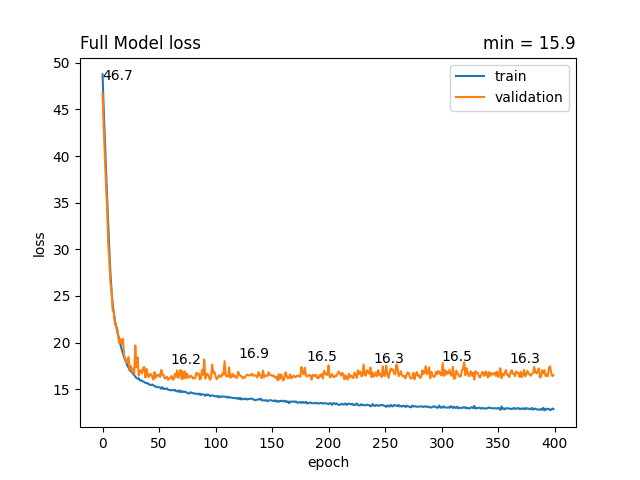
\includegraphics[width=0.5\textwidth]{400_loss}
    \caption{Initial experiment loss (400 epochs on Wiki)}
    \label{fig:400_loss}
\end{wrapfigure}

An initial experiment was performed by training the C3AE model for
400 epochs on the Wiki dataset as a means to test the \texttt{tensorflow} environment
and the functioning of the implemented C3AE model within it.

The evolution of training and validation loss is shown in \autoref{fig:400_loss}.
The experiment ran to completition with no runtime errors, and
it can be observed that the model was able to decrease its loss,
and that such loss reached an asymptote around epoch 50.

For this reason, we concluded that a training time of 400 epochs
is too much for this model and decided to set the epoch limit to 100 for
all following experiments, assuming that they would have a similar
evolution to this one and therefore all significant improvement
would happen much before the 100\textsuperscript{th} epoch,
in order to reduce the experiments' computation time.

\section{??other full experiments??}
????????????????????????

(One on Wiki, one on UTK, one on Wiki+UTK, all tested w/ FGNET)

????????????????????????

\section{Ablation Study}
A separate set of experiments was performed to study the impact on performance
of the following components of the model and the training process:
the context module and the cascade module of the C3AE model,
and the training data augmentation.

We trained the following variants of the full C3AE model:

\begin{itemize}
  \item \textit{Full model}: the standard model with no changes,
    to serve as a benchmark against the other variants.
  \item \textit{No augmentation}: the data augmentation transformations
    on the training data are disabled.
  \item \textit{No context}: the context module of C3AE is excluded.
    Therefore, only one crop, the outermost one, is given as input to
    the model, and obviously there is no concatenation phase.
  \item \textit{No cascade}: the cascade module of C3AE is excluded.
    Consequently, the intermediate layer between the concatenated feature vector
    and the age output loses its meaning of two-point representation of age
    and becomes a plain hidden layer. This also means that this variant
    does not compute any KL Divergence and outputs only the final age estimation;
    the loss depends only on the age MAE as well.
  \item \textit{No context and no cascade}: both modules are disabled.
\end{itemize}

Each variant was trained for 100 epochs on the Wiki dataset.
((Use of test set needs some debugging))

((plot and discuss results))


%!TEX root = report.tex

\chapter{Project structure}
Probabilmente non ci serve, ma non voglio scordarmi che esiste

%!TEX root = report.tex

\chapter{Conclusions}

\begin{center}
    \begin{tabular}{||c | c c c c c||}
    \hline
    Model & Dataset & Augmentation & Epochs & Validation MAE & Test MAE\\ [1ex]
    \hline\hline
    Full & Wiki & × & 100 & 8.36 & 24.41 \\ [1ex] 
    \hline
    Full & Wiki & Some & 400 & 6.82 & 22.72 \\ [1ex]
    \hline
    Full & Wiki & \checked & 100 & 6.79 & 18.11 \\ [1ex]
    \hline
    Full & UTK & \checked & 100 & 8.67 & 9.79 \\ [1ex]
    \hline
    Full & Wiki + UTK & \checked & 100+100 & 8.23 & 8.64 \\ [1ex]
    \hline
    Full Ablation & Wiki & \checked & 100 & 12.60 & 18.69 \\ [1ex] 
    \hline
    No Cascade & Wiki & \checked & 100 & 12.60 & 18.67 \\ [1ex] 
    \hline
    No Context & Wiki & \checked & 100 & 6.88 & 20.73 \\ [1ex] 
    \hline
   \end{tabular}
\end{center}

%\begin{figure}[!ht]
%\centering
%    \includegraphics[width=300pt]{images/prova.png}
%\end{figure}



\bibliography{bibliography}
\bibliographystyle{ieeetr}

\begin{thebibliography}{100}

	\bibitem{prova} {Pippo, Pluto e Paperino. Guida di Paperopoli. ICLR, 1050:11, 2021}

	% [Francesco] Prevedo problemi di merge in questa sezione,
	% quindi rendo più esplicito che mai che
	% QUESTE SONO LE CITAZIONI CHE AGGIUNGO PER IL CAPITOLO 2
	\bibitem{wiki}{
		Rasmus Rothe and Radu Timofte and Luc Van Gool.
		\textit{Deep expectation of real and apparent age from a single image without facial landmarks}.
		IJCV 126(2-4):144–157, 2016.
	}
	\bibitem{fgnet}{
		Yun Fu, Guodong Guo, and Thomas S Huang.
		\textit{Age synthesis and estimation via faces: A survey}.
		IEEE Trans. on Pattern Analysis and Machine Intelligence 32(11):1955–1976, 2010.
	}
	\bibitem{mtcnn}{
		Kaipeng Zhang, Zhanpeng Zhang, Zhifeng Li, Yu Qiao.
		\textit{Joint Face Detection and Alignment using Multi-task Cascaded Convolutional Networks}.
		IEEE Signal Processing Letters 23(10):1499–1503, 2016.
	}
  \bibitem{random_erasing}{
    Zhun Zhong, Liang Zheng, Guoliang Kang, Shaozi Li, and Yi Yang.
    \textit{Random erasing data augmentation}.
    arXiv preprint arXiv:1708.04896, 2017.
  }
	% FINE DELLE CITAZIONI CHE AGGIUNGO PER IL CAPITOLO 2
	% rimuovere questi commenti quando siamo sicuri che il merge è andato bene
\end{thebibliography}


\end{document}
